\chapter{Visualisation Evaluation}\label{C:eval}
Following the completion of the implementation of IKVT a final
user evaluation was carried out. This evaluation was
 designed to discover whether the implemented visualisation
successfully fulfilled the requirements of the project. The evaluation
was a within subjects experiment conducted with 10
participants. This means that all participants were exposed to every condition
in the experiment. Each participant took turns using the IKVT with both keyboard
\&
mouse and Kinect sensor whilst answering a set of questions.
The evaluation was designed to qualitatively and
quantitatively assess users
reactions and experiences with the IKVT. By mapping the experiences of users to
the
project requirements it was possible to evaluate the success of IKVT. The choice not to perform comparative evaluation against other existing visualisations was made for three main
reasons; (1.) new features were being implemented that no previous
visualisations had, (2.) the inclusion of interaction via gesture was intended
as a proof of concept and so users experiences were important, and (3.) The goal
of the evaluation was to evaluate IKVT against the project requirements.

\section{Purpose of Evaluation}
User studies offer a 
scientifically sound method to measure the performance of a visualisation.
Studies can 
be used to evaluate the strengths and weaknesses of 
different visualisation techniques or show that a visualisation technique is 
useful in a practical sense, according to some objective 
criteria, for some specific task \cite{kosara2003thoughts}. 
The fundamental goal of conducting user studies is to 
seek insights into why particular visualisation techniques are effective
\cite{kosara2003thoughts}.


\section{Experimental Design}
\subsection{Expectations of Evaluation}
An expectation in this evaluation was that users would take approximately three
minutes to feel comfortable with using the visualisation for the basic tasks of
moving the camera around, sorting the exoplanets, and using the range sliders to
filter the exoplanets. 

Following this acclimitisation time it was expected that users could accurately
complete the set of questions in a worksheet (APPENDIX QUESTIONS) whilst using
the visualisation. During this stage users were expected to use both interaction
methods (Keyboard \& Mouse, and Kinect sensor). It was predicted that during the
keyboard \& mouse
portion of the experiment the users should make more accurate selections and
exhibit more effective data seeking behavior, whereas during the Kinect portion
they would be more interested in experimenting with gestures rather than
attempting to gain information about exoplanets.

When users have finished using the visualisation and fill in the questionnaire
asking them about their experience. The expectation was that
they would detail the areas of the visualisation that they had trouble with,
felt needed improvement, and that they found useful and fun. These two forms of
results gathering provided both qualitative and quantitative results describing
the
users experiences.
The expectation was that these qualitative and quantitative user results would
provide a means of viewing how successful the visualisation was in terms of
fulfilling the system requirements.

\subsection{Participants}
The user study was undertaken by 9 participants referred to as P2 through P10 as
well
as  
a pilot study by a single participant referred to as P1. All were either
students
or
young professionals from a mix of specialties, aged between 21 and 26 and a
mix
of genders with 5 females and 4 males. 6 of these participants had extensive
prior experience with Kinect sensors, and all participants had experienced a 3D
visualisation before. 6 out of the 10 participants had knowledge of the
exoplanets discovered by the Kepler telescope. These are shown in the following
table in Figure \ref{fig:participanttable}
\begin{figure}[H]
  \centering
      \includegraphics[width=0.8\textwidth]{images/participanttable.pdf}
  \caption[Summary of participants]{This table displays the attributes of each
of the participants in the evaluation.}  
    \label{fig:participanttable}
\end{figure}

\subsection{Evaluation Environment}
The environment of the evaluation was set in a closed computer laboratory of
twelve computer stations. One duel monitor PC was set asside for the evaluation.
This PC had an i7 processor, 8gb ram, and was running KDE \cite{kde} as the
opperating system.  


\begin{figure}[H]
  \centering
      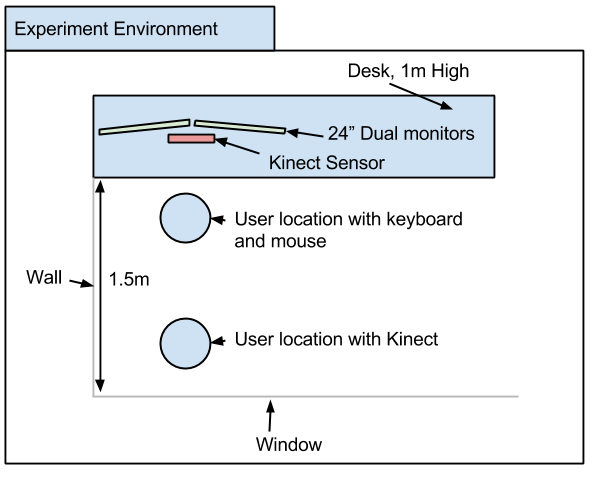
\includegraphics[width=0.8\textwidth]{images/environment.png}
  \caption[Image of evaluation environment]{Image of evaluation environment showing the seating positions and hardware locations.}  
    \label{fig:environment}
\end{figure}


\begin{figure}[H]
  \centering
      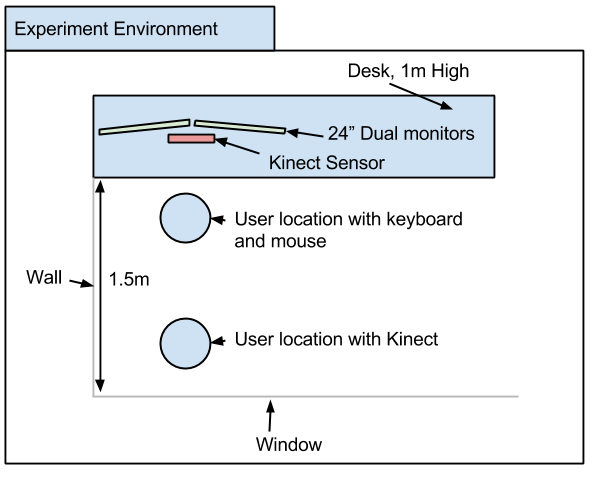
\includegraphics[width=0.8\textwidth]{images/environment.png}
  \caption[Evaluation environment plan]{Evaluation environment plan showing layout of all hardware components.}  
    \label{fig:environment}
\end{figure}


\subsection{Evaluation Method}
A poorly designed experiment will only yield results of limited value, because
of this it was important to ensure that each stage of the experiment was
focused on evaluating a specific area of the visualisation in relation to the
project requirements \cite{stasko}. There were three key methods of gathering results during
this
evaluation; a
worksheet to fill out whilst using the visualisation made up of two sets of
questions (one for the keyboard \& mouse system and one for the Kinect
system)(APPENDIX), a questionnaire to
fill in afterwards about the experience (APPENDIX), and the examiners
observations about
how the users interacted with the system.  
\\\\
The following are the steps that were carried out during each user evaluation to
ensure that the variables were the same each time
\begin{enumerate}
\item The participant enters the room and sits down at the computer.
\item They are handed the consent form and information sheet.
\item After these are completed they are handed the user questionnaire and the
set of questions to answer while using the system. On this questionnaire there
are two sets of questions, the first is for the keyboard \& mouse system, and
the second if for the Microsoft Kinect system.
\item They are then given a brief introduction into each of the visualisation
components and what the visualisation as a whole represents
\item Following this they are advised that they have 5 minutes to get
familiarised with the system but they do not need to use all of this time (the
amount of time taken will be recorded for analysis of how user friendly and
intuitive the system is).
\item Following this the participant is asked to complete the worksheet by first
using the mouse and keyboard system. When they feel they have answered the first
set of questions they will notify the examiner who will move the user to the
Kinect
system to continue with the second set.
\item Once the participant has completed both sets of questions they are asked
to fill
in the qualitative user questionnaire about their experiences using the
visualisation. 
\item Following this if the examiner has no follow up questions the user is free
to leave.
\end{enumerate}

\subsection{Pilot Study}
Due to the significant financial and resource costs associated with running an
experiment, it 
is valuable to conduct a pilot study with one or two 
participants. This allows testing and refining of the experimental
design before starting a full-fledged study with numerous 
participants \cite{kosara2003thoughts}. 

The reason for conducting a pilot study for this project was to ensure that
the experiment was producing the data needed to evaluate IKVT as well
as taking the correct amount of time to complete. It was also
used to discover whether any aspects of the study would
interfere with the results. One participant was asked to take part in a pilot
study, this participant is referred to as P1. P1 was asked to complete all of
the activities that
make up the main experiment. This pilot study took approximately 15 minutes as
intended including the time needed for the explanation and completion of
paperwork, as well as the experiment itself.

P1 successfully completed each of the questions in the worksheet whilst using
the visualisation with only
limited assistance from the examiner. This assistance was required due to the
wording of
some of the tasks being ambiguous causing
unnecessary confusion which could have interfered with the results. These
ambiguous questions and
tasks were removed prior to the main user study. During the main study only P4
and P10 asked for clarification on the questions or tasks.

P1 had some initial difficulty using the range sliders but after a small period
of experimentation began using them for the majority of tasks which turned out
to be effective. P1 also found that whist the range sliders were useful,
they did not allow fine enough control for making small changes to the filters.
The component
of the visualisation that P1 had the most difficulty with was using the
Goldilocks
view. This difficulty seemed to stem from the lack of a common point of
reference for each planet due to each planet having a different star with its
own Goldilocks zone.

During the Kinect portion of the experiment P1 found that being in a sitting
position whist interacting with the visualisation did not feel natural due to
``being required to reach out and exert effort to hold an upright position of
the arms for an extended period of time''. The following figure displays P1s
quantitative results from the questionnaire.
\begin{figure}[H]
  \centering
      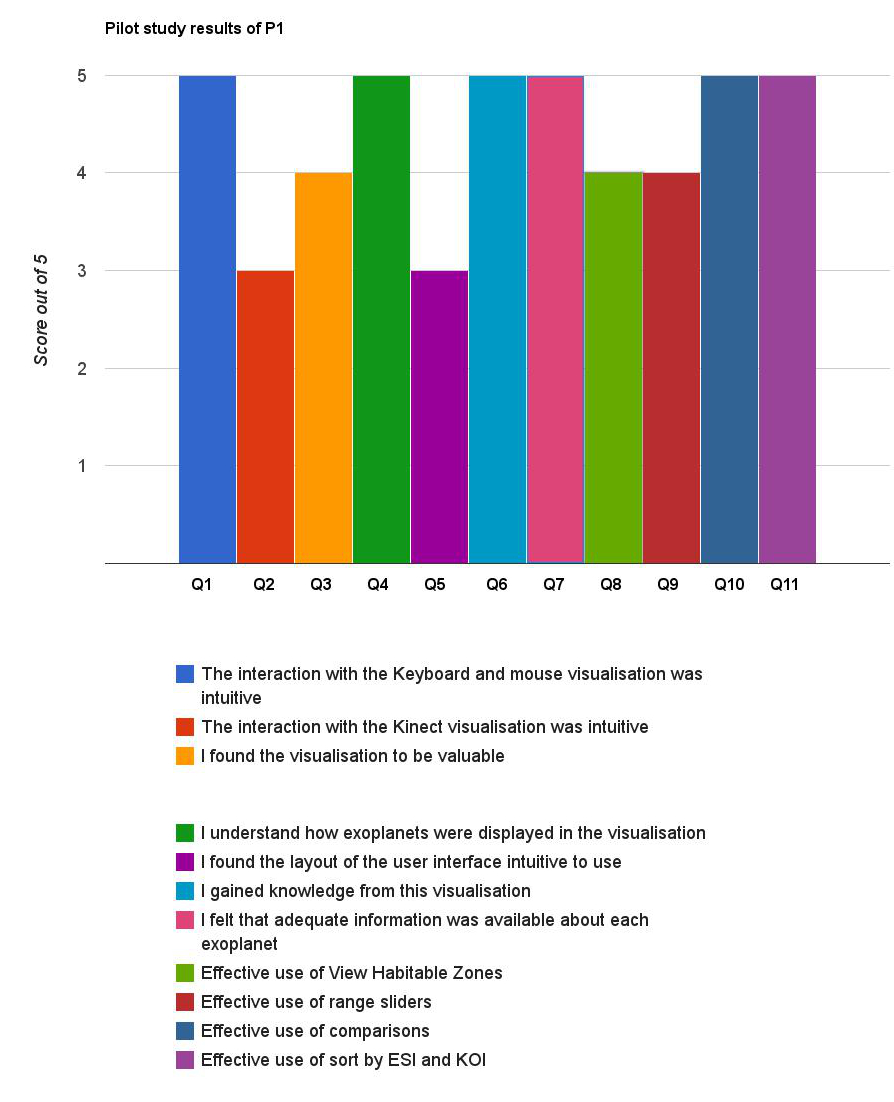
\includegraphics[width=1\textwidth]{images/pilot.jpg}
  \caption[Pilot study results]{Pilot study quantitative results of P1. Points
of interest in this graph are that Q2: The Kinect visualisation was intuitive,
and Q5: I found the layout of the user interface intuitive to use, both scored
lowly but The interaction with keyboard and mouse was intuitive and P1 was still
effectively used the visualisation.}  
    \label{fig:pilot}
\end{figure}

\section{Results of Evaluation}
The keyboard \& mouse portion of the experiment was primarily intended to
evaluate how the interaction techniques introduced into the
visualisation aided users in their information seeking behavior.
This was evaluated through the first part of the worksheet filled
in by users whilst using the visualisation. These questions were designed in a
way that
encouraged users to make use of each of the interactive features that was
implemented as part of this project.

The Microsoft Kinect portion of the experiment was intended to evaluate how
users would react to interacting with the visualisation by gesture. The
worksheet for this portion of the evaluation were designed to find out whether
users could successfully navigate the visualisation without keyboard \& mouse.
The following subsections discuss the qualitative and quantitative results of
this evaluation. 

\subsection{Qualitative Results}
This subsection discusses the qualitative and quantitative results returned by
the user evaluation.
\subsubsection{Evaluation of Functional Requirements}
\begin{enumerate}
{\bf
 \item[R1.] The visualisation needs to display planetary information to convey
knowledge to users.}

The experiment demonstrated that the increased amount of information available
in IKVT
 about each exoplanet allowed participants to access
more information contained in the Kepler Exoplanet database than in the previous
system. All participants were able to successfully complete the worksheet
questions
that involved accessing information about exoplanets stored in the
text areas in the control panel.
P8 found that a weakness of the system was the amount of concepts that needed
to be understood about exoplanets and so including a glossary would be an
improvement. A glossary would allow users to discover the meaning to any terms
in the visualisation mitigating the risk of user
confusion.

All participants reported learning something from the visualisation that they
did not previously know, and those who had no knowledge of exoplanets prior to
the experiment felt that they had learned something valuable. For example P4
felt that using IKVT broadened her perception of how much information we know
about planets so far away.


{\bf
 \item[R2.] The visualisation needs to allow exoplanets to be compared against
one another.}

Whilst all participants used the comparison functionality during the
familiarisation stage, only three of the participants (P3, P8, P10) used it
while completing the
worksheet. This could be because it was not made obvious enough, or because the
questions asked of users did not force users to use this feature to get an
answer. When the participants did use the comparison tool they were able to use
it successfully and most tried it multiple times with multiple exoplanets. P3
found that being able to compare the exoplanets against one another was useful
as he could leave an interesting exoplanet selected whilst comparing it against
multiple other exoplanets. He found that it was easy to compare the information
for each exoplanet and to get a sense of the attributes of exoplanets.

{\bf
 \item[R3.] The planets need to be able to be ordered by their similarity to
earth (ESI) and by their Kepler Object of Interest number (KOI).}
 
All participants used the sort by KOI and ESI functionality effectively without
any confusion. P8 liked being able to toggle between the different attributes
sortings as he found that it gave a clearer view of the attributes in a visual
manner rather than needing to look at the text areas.
P7 found the exoplanets sorted by ESI to be the most interesting view. She
spent an extended period of time experimenting with this during question 8 of
the
worksheet before moving on the later questions. P7 stated that she could find
the potentially habitable planets easily as she could see that they were similar
to Earth which was displayed clearly.

{\bf \item[R4.] The visualisation needs to allow users to define ranges of
planetary attributes to filter which planets are displayed.}

All participants successfully used the range sliders whilst completing the
worksheet questions. The range sliders were used frequently by all participants
to discover the
exoplanets that were the outliers in regard to their attributes (i.e. high
temperatures). 3 out of 10 participants had trouble when moving between
questions on the worksheet due to forgetting
to reset the range sliders after using them and thus only a subset of the
exoplanets were displayed. 
P5 found the zooming effect that occurred when planets were filtered useful for
making more accurate selections and spent time
experimenting with it. P6 found that being able to sort the planets according to
attributes and
then filtering them to remove the planets she did not want was a powerful tool.

{\bf \item[R5.] Users need to be able to view the habitable zones (Goldilocks
zones) of stars in
relation to the planets orbiting them.}

The evaluation of this requirement showed that whilst the functionality was
successfully implemented it lacked usability. All but one user in the study
found that this was because it was unintuitive. What caused this was that the
Goldilocks zone of each star is different. This meant that each time a user
selected a new exoplanet the location of each of the zones changed as was
intended. This confused all but one user (P10) as they were expecting the
zones to stay the in the same locations.  

\end{enumerate}

\subsubsection{Evaluation of Nonfunctional Requirements}
\begin{enumerate}
 {\bf\item[R6.] All interaction methods must be visible and intuitive.}
 
The experiment found that all interactive methods were able to be seen and used
by users. However due to the design of the components being low key as to not
draw attention away from the main visualisation, the participants often forgot
about them, especially as the control panel was at the side of the screen.
For example, P5 found that because the information panel was not central in the
visualisation
it required effort to break away from the main visualisation window and thus
broke
the immersion. Another issue found was that the text of the components in the
interaction was too small for some users to see clearly and quickly.
A common consensus was that the layout of the interactive components were fine
but could be improved by making them ``pop out more'' (P10) especially as many
participants didn't initially spot the text areas changing as planets were
selected
until reading the worksheet questions.
 
{\bf \item[R7.] The visualisation must remain uncluttered to reduce information
overload.}

All users felt that the amount of information displayed in the
visualisation was appropriate apart from P7 who felt
it displayed to much information at once which caused confusion. P10 felt that
the control panel contained the right amount of information, but felt that
it could be improved by changing its design to make it stand out more and
emphasis each component contained in it. P4 felt that the names of some of the
attributes were not made clear enough (E.g. ESI, KOI). P5 felt that limiting the
amount that the camera could move would be an improvement,
especially in the graph view where their is a fixed plane where content is
displayed.

{\bf \item[R8.]  There needs to be two modes of interaction in the system,
keyboard \& mouse vs gesture based.}

\begin{figure}[H]
  \centering
      \includegraphics[width=0.8\textwidth]{evaluation/fra.jpg}
  \caption[Participant using Kinect visualisation]{Participant using Kinect
visualisation performing selection of an exoplanet}
  \label{fig:fra}
\end{figure}

The experiment found that both the interactive mediums had different
strengths and weaknesses. The keyboard \& mouse system was the most effective
for information seeking as it provided more accuracy and was easier to use the
control panel elements. The Microsoft Kinect system was worse for discovering
information, but it was the most fun out of the two options due to its novelty.
All of the users felt that had they had more time with the Kinect system, they
would have been more effective at accessing the information available. This was
because they were preoccupied performing basic actions like moving the camera
and selecting planets due to the short time available. For example P6 found that
she used more time playing around with the Kinect system trying to select
planets rather than trying to get information. All participants but P4 felt that
the visualisation responded with the appropriate actions and magnitudes for each
gesture. P4 expected the magnitude of the visualisation changes to be more
than they were, ie it should have rotated faster. P6 felt that there needed to
be more physical movement space in which to use the Kinect as some movements
felt
cramped. Another weakness discovered about the Kinect sensor was that it
detected the whole hand rather than a more controllable area like a finger.
P10 found that overlapping planets made it hard to make selections with the
Kinect and that he needed a way to cancel a selection without having to select
another planet.

\end{enumerate}

\subsection{Quantitative Results}
\subsubsection{Evaluation of Functional Requirements}

A key part of this visualisation is that it should be intuitive enough that a
user can walk up to it and feel comfortable using it to explore data within a
short period of time. The results showed that some users felt that they could
effectively use the visualisation very quickly (within 1 to 4 minutes) whilst
others took longer (up to 5 minutes) as Figure \ref{fig:comfort} shows. 
\begin{figure}[H]
  \centering
      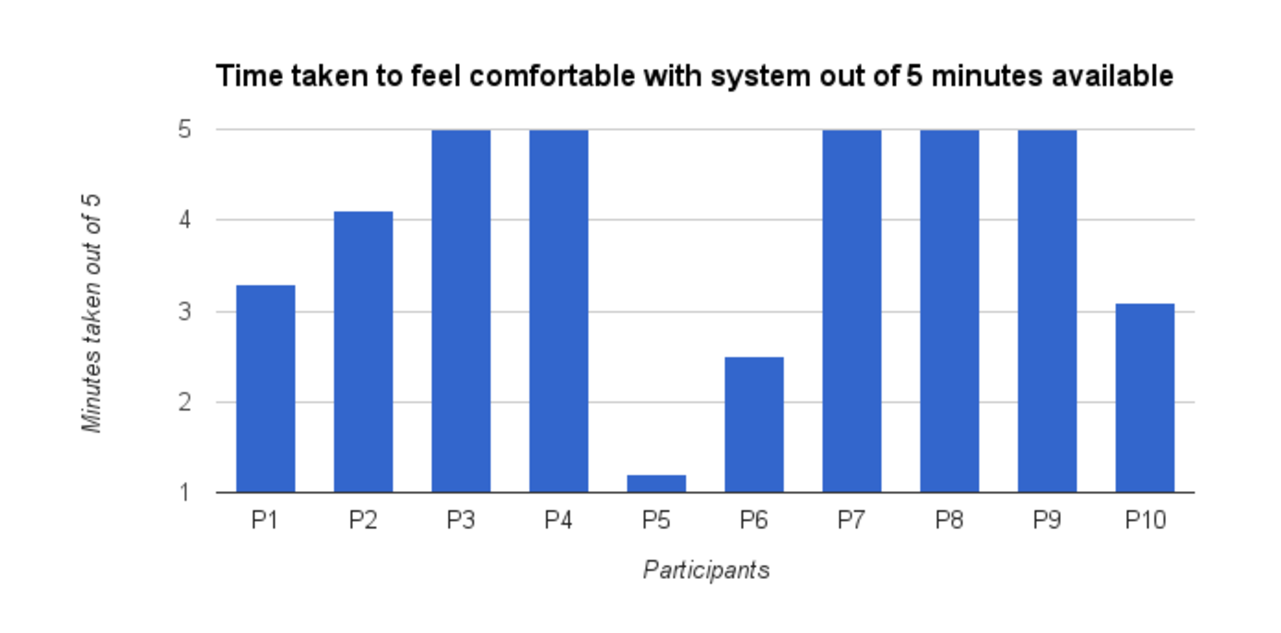
\includegraphics[width=1\textwidth]{images/comfort.pdf}
  \caption[Time taken to feel familiar with IKVT]{Amount of time taken out of a
possible 5 minutes for users to feel
comfortable with
visualisation before moving onto the worksheet. A notable reult from this is
that even though P5 took the shortest amount of time, he was also very
successfull while using the visualisation as shown in Figure
\ref{fig:breakdown}. This could mean that some users will naturally find the
visualisation easier to use than others like P4 who took the full amount of time
and still had trouble IKVT}  
\label{fig:comfort}
\end{figure}

As we can see below in Figure \ref{fig:summary}, all users performed well in all
aspects apart from with ``Req: 5 Effectively used habitable zones'' which the
qualitative analysis also found. Another notable result was that the keyboard \&
mouse was rated as more intuitive than the Kinect sensor, again this is
supported by the qualitative results. Apart from these key areas of interest the
results are as expected with each area being scored highly. 
\begin{figure}[H]
\centering
      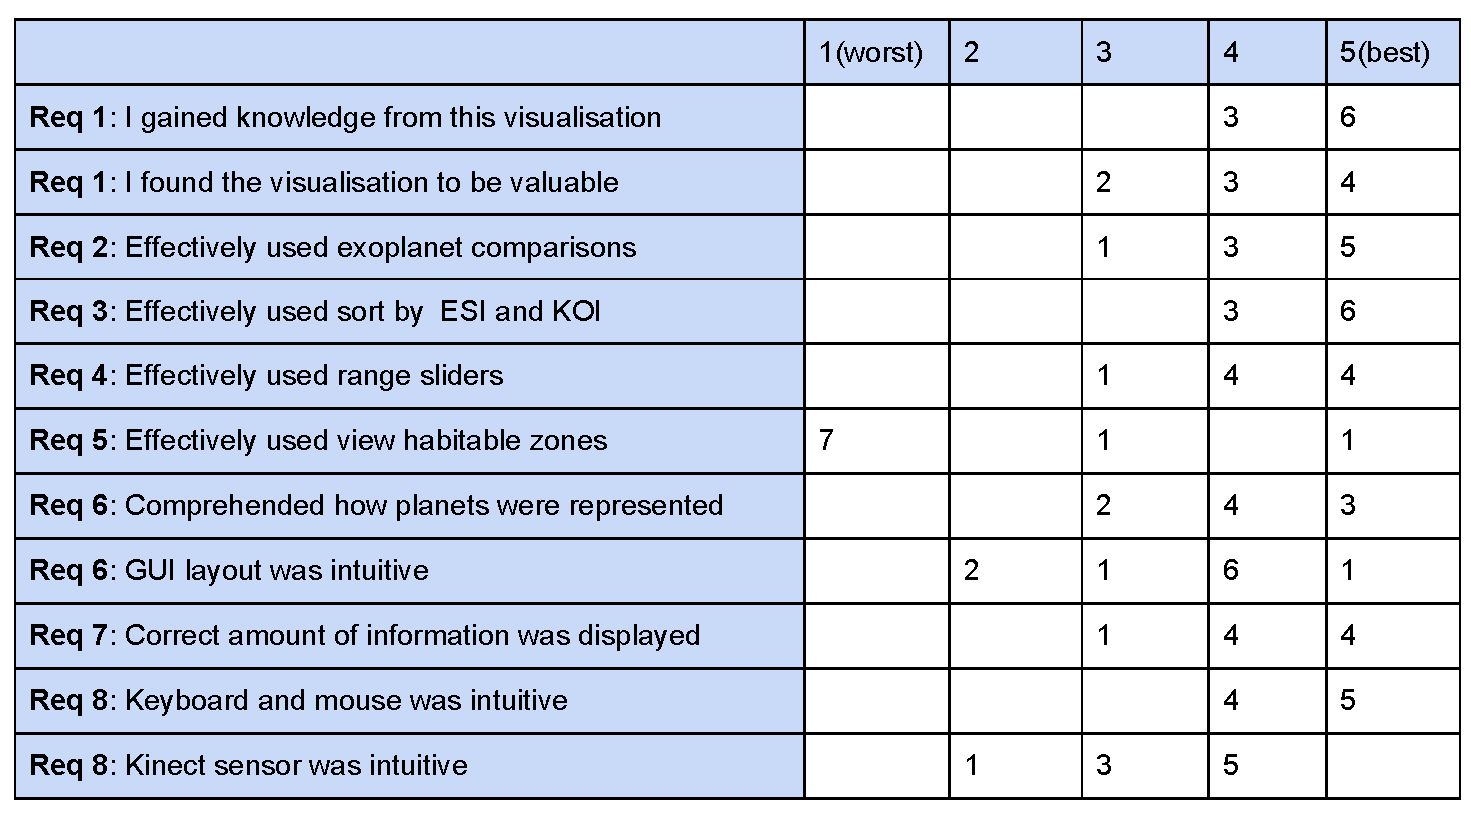
\includegraphics[width=1\textwidth]{images/summaryResults.pdf}
  \caption[Summary of the quantitative results]{Summary of the quantitative
results gathered from participants. Notable points are the negative responce
surrounding Requirement 5 which matches the qualitative results. Apart from this
all other areas scored highly.}  
    \label{fig:summary}
    \end{figure}
    
Seeing how different participants scores attribute to the table in Figure
\ref{fig:summary} helps to understand the distribution of scores. As Figure
\ref{fig:breakdown} shows, some users consistently gave higher or lower scores
which could have caused a bias in the results. However it does show that some
users enjoyed using the visualisation whilst others did not. 
    
\begin{figure}[H]

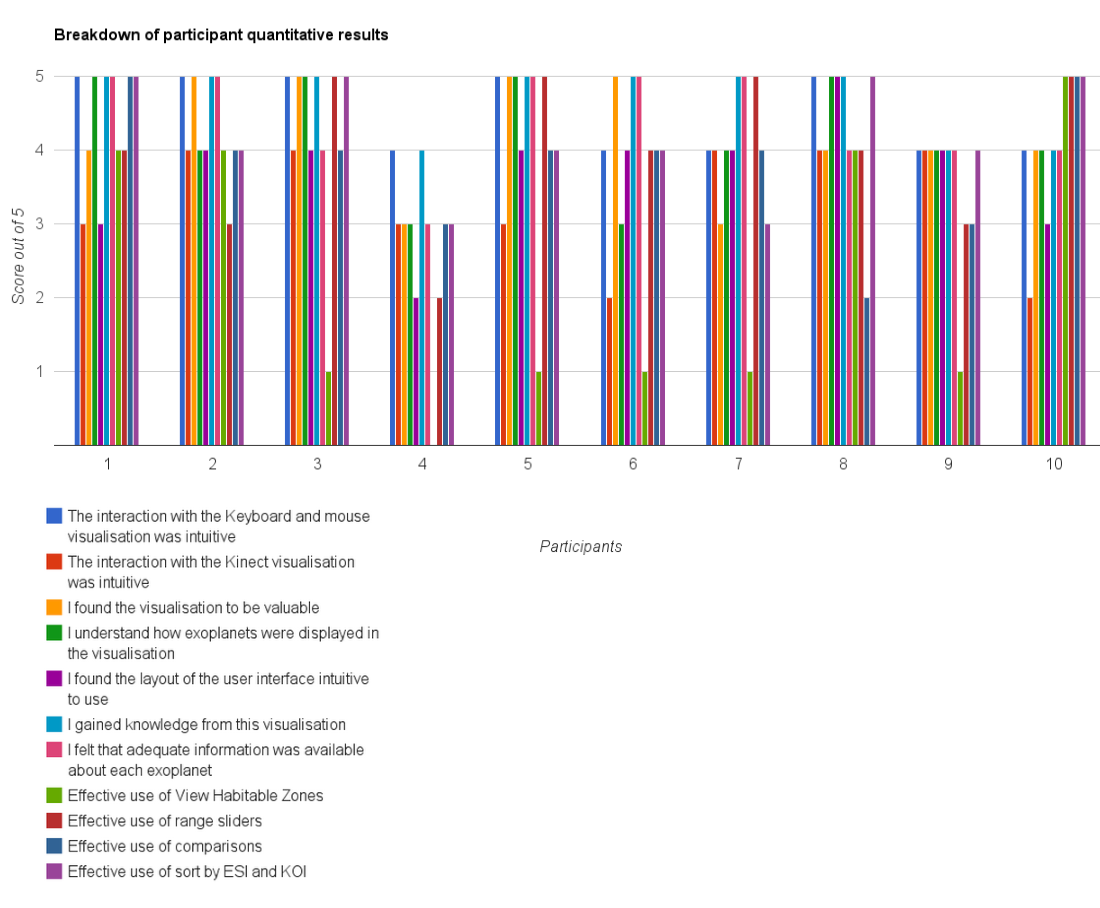
\includegraphics[width=1.3\textwidth,angle=90]{images/breakdown.pdf}
  \caption[Summary quantitative results]{Summary of quantitative results between
users. A notable finding is that some users consistently gave higher or lower
scores
which could have caused a bias in the results. It also showed that some users
enjoyed the visualisation more than others.}  
    \label{fig:breakdown}
\end{figure}



\section{Discussion}
\subsection{Threats to Validity}
A key factor in this user evaluation was the small number of users
chosen due to the time limit of 300 hours which did not allow for a larger and
more
in depth study. Because of this, the results gathered may
not be representative of a larger population. It was also limited to a narrow
demographic of young professionals and students which does not cover all of the
intended users of IKVT. To amend this, the population of this study would need
to
be expanded to contain age ranges above and below those in this study.

A further threat to the validity of this evaluation was the limit placed on
participants for the familiarisation stage. Some participants may have required
even more time than the 5 minutes alloted for. By cutting the familiarisation
stage off at this point it may have caused some participants to be unprepared
to complete the worksheet and thus skew the results.

\subsection{Potential Improvements}
Due to the negative results surrounding the viewing of Goldilocks zones,
this area of the evaluation should be analysed further to determine whether the
tasks in the evaluation relating to it were flawed, or whether the functionality
and its design were flawed. To discover this it would be important to evaluate
the questions used in the study to determine whether or not they skewed the
result or if the the functionality needs to be
redesigned. 


\section{Summary of Evaluation}
This evaluation of IKVT provided several key results and insights into the
success of IKVT. The general consensus by the participants of the study
was that the system had a low learning curve, was enjoyable to use, and allowed
access to interesting information. Participants also agreed that the Kinect
system was more fun to use than the keyboard \&
mouse because of its novelty, but lacked the control that the
keyboard \& mouse allowed which made it less effective at accessing the
information in the visualisation. The keyboard \& mouse was found to the be the
most effective method for navigating the visualisation because of the amount of
control that it offered users as well as being the interactive medium that
participants had the most experience with.

The evaluation revealed one problem area in the visualisation that was related
to Requirement 5 (Users need to be able to view the habitable zones of stars in
relation to the planets orbiting them), and Requirement 6 (All interaction
methods must be visible and intuitive). This problem occurred because users
found that
viewing where each exoplanet was located in relation to their stars habitable
zones was unintuitive and difficult to use. This result could have occurred for
a
range of reasons, the most likely being that the evaluation questions were
counterproductive to using this functionality, or that the functionality itself
is flawed.

This user study served to evaluate how effectively IKVT could convey the
information in the Kepler Exoplanet dataset. The findings pointed to it
being successful in this regard. However, there are areas that this evaluation
could be improved to strengthen this result. The main improvement for this
evaluation is to include a larger number of participants more representative of
the wider population. These results were first gathered in the qualitative
study, and were then confirmed by the quantitative results that found the same.



